%\subsection{SystemML \textit{quantile} Algorithm}

%Based on the rationality described before, we developed an sort-based \textit{quantile} algorithm. 
%\subsection{Sort-Based Order Statistics Algorithm} \label{sec:sort-order-stats}

\onefigure
{figs/orderStats.eps}
{Sort-Based Order Statistics Algorithm}
{fig:orderStats}

%\begin{figure}[t]
%\centering
%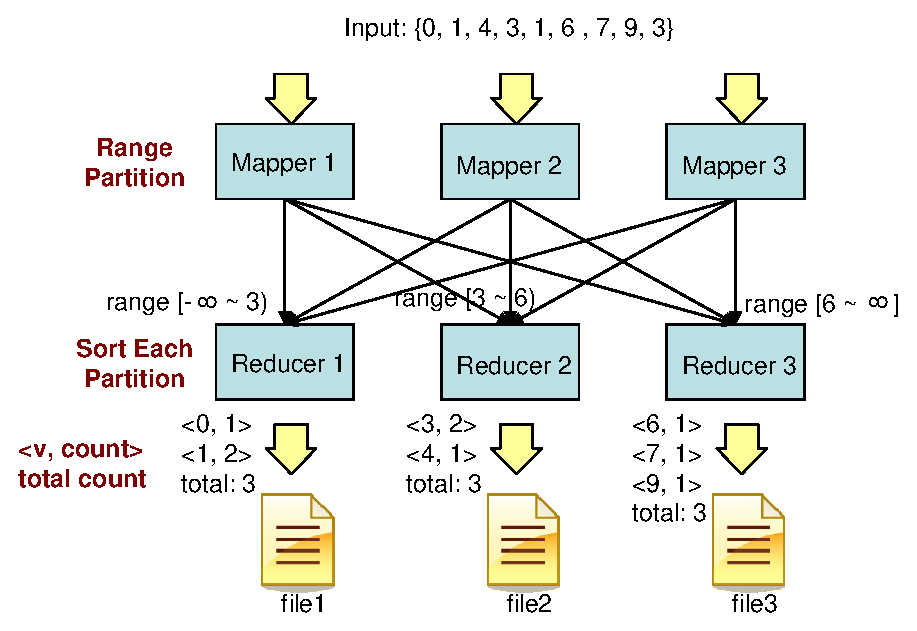
\includegraphics{figs/orderStats.eps}
%\caption{Sort-Based Order Statistics Algorithm}
%\label{fig:orderStats}
%\end{figure}

\textbf{Sort-Based Order Statistics Algorithm:} This algorithm consists of three phases. The first two phases are inspired by Yahoo's TeraSort algorithm~\cite{terasort}.

%This algorithm has the following three phases: (1) the sample phase to decide on the boundaries for range partitioning the data, (2) the sort phase to sort each range partition, and (3) the selection phase to select the order statistics. The first two phases are very similar to Yahoo's TeraSort algorithm~\cite{terasort}.

%\textit{Sample Phase}: This phase samples $N_s$ data items from the input data in a serial program. The $N_s$ samples are then sorted and divided evenly into $r$ partitions, where $r$ is the number of reducers allocated. The pivots of the sample partitions are used as the boundaries for range partitions in the next phase.

% more detailed description of the sampling phase.
%Given a specified number of samples $N_s$ and the proportion of the HDFS blocks to be touched for the sample $p$, this program randomly selects $p*B$ ($B$ is the number of HDFS blocks for the input data) blocks, and samples $N_s/(p*B)$ data items from each block. Then, the sample is sorted and divided evenly into $r$ partitions, where $r$ is the number of reducers allocated for the \textit{quantile} algorithm. The pivots of the sample partitions are used as the boundary for range partitioning the whole input for the next phase.


%\textit{Sort Phase}: This phase is implemented as a MapReduce job. The job reads the input data, and uses the results from the sample phase to range partition the input data, each reducer corresponding to one range. Each reducer sorts the unique values in their ranges and also keep a count for each unique value (a similar combiner is used to reduce the data shuffled to the reducers). In addition, each reducer computes the sum of all the counts (i.e. the number of data items) in its range.

%\textit{Selection Phase}: The sort phase produces $r$ sorted HDFS files, as well as the number of data items in each file. It is straightforward to derive which file contains a given order statistic. Locating the order statistic requires only scanning this file until the data item is found (early termination is possible). When multiple required order statistics reside in a single file, the scan cost can be shared. In addition, different files are scanned concurrently to improve further efficiency.

%Then, the algorithm scans the file until it finds the required data item(s). If multiple quantiles reside in the same HDFS file, the scan cost can be shared. When the input quantile vector $P$ is very large and the algorithm has to touch multiple HDFS files to compute all quantiles in $P$, we implement a special Hadoop InputFormat class to perform the selection phase, with each input split scans one file until all required data items are reached and feeds the quantiles directly to whatever jobs that use this input format. 

%\reminder{how about describing the way to do all columns at once? Not sure, because, right now the quantile is only defined on a vector}


\textit{Sample Phase}: This phase samples $N_s$ items from the input data, which are then sorted and divided evenly into $r$ partitions, where $r$ is the number of reducers. The boundary points are used for range partitioning in the next phase.

\textit{Sort Phase}: As shown in Figure~\ref{fig:orderStats}, this phase is a MapReduce job that reads the input data, and uses the results from the previous phase to range partition the data. Each range is assigned to a different reducer, which sorts the unique values and keeps the number of occurrences for each unique value. Each reducer also computes the total number of data items in its range.

%\textit{Selection Phase}: The output of sort phase ($r$ sorted HDFS files and their sizes) is be used to identify the appropriate file(s) for the required order statistic(s). If multiple statistics reside in a single file, the scan cost can be shared. Furthermore, different files are scanned concurrently for improved efficiency.

\textit{Selection Phase}: For a given set of required order statistics, the output of sort phase ($r$ sorted HDFS files and number of items in each file) is used to identify the appropriate file(s) that need to be scanned. If multiple order statistics reside in a single file, the scan cost can be shared. Furthermore, different files are scanned concurrently for improved efficiency.


%The sort phase produces $r$ sorted HDFS files, as well as the number of items in each file. It is straightforward to derive which file contains a given order statistic. Locating the order statistic requires only scanning this file until the data item is found (early termination is possible). When multiple required order statistics reside in a single file, the scan cost can be shared. In addition, different files are scanned concurrently to improve further efficiency.
